\chapter{Framework}
\minitoc% Creating an actual minitoc

\par In the previous chapter, we set the foundations of studying styles, which is the work done in the PhD. We explored our choices for generative models and the evaluation metrics, and how to ground them. We also had a discussion about lower- and upper-bound benchmarks. These foundations are necessary in order to have baselines to compare to, and performance aspects (i.e., metrics) use for this comparison. \OSM{write a note about the fairness of selecting the baselines, and the reasoning behind them.}

\par In this chapter, we build on these foundations, by proposing the use of conditional temporal auto-encoder framework in order to study and extract styles, in the context of sequences (i.e., a time aspect exists in the data). We take advantage from the fact that the content is well known in our dataset (i.e., the identity of the letters in IRONOFF, and the identity of the shapes in QuickDraw!).

\begin{mdframed}[backgroundcolor=blue!20]
    \begin{center}
        Questions addressed in this chapter
    \end{center}

    \setlist{nolistsep}
    \begin{itemize}[noitemsep]
        \item What possible framework to study styles? and why?
        \item How does this framework performance compare to the benchmarks?
        \item What kind of styles we can extract from this framework? and how do we extract them?
    \end{itemize}
\end{mdframed}

\section{Background}
  \subsection{Auto-encoders}\label{sec:autoencoder}
  \setlist{nolistsep}\begin{itemize}[noitemsep]
      \item General intro about auto-encoders
      \item Applications of static auto-encoder in image Reconstruction
      \item Temporal auto-encoder
      \item different ways to bias temporal encoders
  \end{itemize}

  \subsection{Objectives}
  \subsection{Static and Temporal auto-encoder}

\section{Putting it all together}
  \subsection{Letter generation with style preservation}
  \par The objective here to compare the quality of the generated letters to the state-of-the-art benchmarks. As mentioned earlier, we compare using the BLEU score metric and the EoS analysis.
  The BLEU score results can be seen in table \ref{table:bleu_gen}, and the results for EoS analysis results are in table \ref{table:EoS_gen}. We can see that the BLEU-3 score results of our model achieves 32.3\% accuracy in Speed feature and 38.7\% accuracy in Freeman feature, compared to 25.1\% and 28.3\% accuracy using the benchmark model on both features respectively.
  \par The same goes for the EoS analysis. In comparing the Person Coefficient, our model achieves 0.99 score compared to 0.55 for the benchmark model (the highest score is 1.0). This is a support that our model capture the style of handwriting better than the benchmark.
  \par Examples for the generated letters can be found in figure \ref{fig:letters_examples}.


  \begin{table*}[!htbp]
  \centering
  \begin{tabular}{|l||c|c|c||c|c|c|}
  \hline
  \multicolumn{1}{|c||}{Aspect/Feature} & \multicolumn{3}{c||}{ Speed } & \multicolumn{3}{c|}{ Freeman }   \\ \hline
  Model / B-score      & B-1  & B-2  & B-3           & B-1  & B-2   & B-3              \\ \hline
  Letter + Writer bias & 51.5 & 41.4 & 25.1          & 56.7 & 39.4  & 28.3             \\\hline
  \textbf{Style Extractor} & 71 & 51.7 & 32.3 & 65.6 & 51.5 & 38.7 \\\hline
  \end{tabular}
  \caption{BLEU scores for different models for known writers.}
  \label{table:bleu_gen}
  \end{table*}

  \begin{table*}[!htbp]
  \centering
  \begin{tabular}{|l||c|c|c||c|c|c|}
  \hline
  \multicolumn{1}{|c||}{Aspect/Feature} & \multicolumn{3}{c||}{ Speed } & \multicolumn{3}{c|}{ Freeman }   \\ \hline
  Model / B-score      & B-1  & B-2  & B-3           & B-1  & B-2   & B-3              \\ \hline
  Letter + Writer bias & 55.4 & 39.6 & 25.3 & 50.2 & 38.6 & 27.7             \\\hline
  \textbf{Style Extractor} & 72.4 & 52.4 & 32.2 & 70.4 & 55.6 & 42.1 \\\hline

  \end{tabular}
  \caption{BLEU scores for different models for style extraction for 30 new writers (style transfer).}
  \label{table:bleu_transfer}
  \end{table*}

  % \begin{table}[!htbp]
  % \centering
  % \begin{tabular}{|l|c|c|}
  % \hline
  % Models & Pearson coefficient & p value \\ \hline
  % Letter + Writer bias & 0.55 & 0.04\\ \hline
  % \textbf{Style Extractor} & 0.99 & 0.01 \\ \hline
  % \end{tabular}
  % \caption{Pearson correlation coefficients and associated p-values for the End-Of-Sequence (EoS) distributions for the different models: a) The results in a normal generation scenario. b) The results on 30 new writers (style transfer).}
  % \label{table:EoS_gen}
  % \end{table}

  \begin{table}[!htbp]
  \centering
  \begin{tabular}{|l|c|c|}
  \hline
  Models & Pearson coefficient\\ \hline
  Letter + Writer bias & 0.55\\ \hline
  \textbf{Style Extractor} & 0.99 \\ \hline
  \end{tabular}
  \caption{Pearson correlation coefficients for the End-Of-Sequence (EoS) distributions for the different models on the normal gene ration scenario}
  \label{table:EoS_gen}
  \end{table}

  % \begin{table}[!htbp]
  % \centering
  % \begin{tabular}{|l|c|c|}
  % \hline
  % Models & Pearson coefficient & p value \\ \hline
  % Letter + Writer bias & 0.5 & 0.7 \\ \hline
  % \textbf{Style Extractor} & 0.99 & 1.4e-29\\ \hline
  % \end{tabular}
  % \caption{Pearson correlation coefficients and associated p-values for the End-Of-Sequence (EoS) distributions for the different models: a) The results in a normal generation scenario. b) The results on 30 new writers (style transfer).}
  % \label{table:EoS_transfer}
  % \end{table}

  \begin{table}[!htbp]
  \centering
  \begin{tabular}{|l|c|c|}
  \hline
  Models & Pearson coefficient\\ \hline
  Letter + Writer bias & 0.5\\ \hline
  \textbf{Style Extractor} & 0.99\\ \hline
  \end{tabular}
  \caption{Pearson correlation coefficients for the End-Of-Sequence (EoS) distributions for the different models on 30 new writers (style transfer).}
  \label{table:EoS_transfer}
  \end{table}

  \subsection{Style transfer}
  \par One of the hypotheses we want to test is whether there is a limited number of styles needed, to generalize over new writers. To achieve this, the learned representation for styles should extract generic information about the styles.

  \par In order to test this hypothesis, we expose our model to 30 writers that have not been seen before. We compare our model performance on these writers with a model is biased by the writer and letter identities (the benchmark model). The latter model was not constrained from seeing those writers (thus, the reported results of the comparison overestimates the actual performance of that model).

  \par The BLEU scores can be seen in table \ref{table:bleu_transfer}. Our model achieves on BLEU-3 score 32.2\% and 42.1\% accuracy on the Speed and Freeman code features, compared to 25.3\% and 27.7\% on the benchmark model for the same features respectively.
  \par The EoS analysis can be seen in table \ref{table:EoS_transfer}. Our model achieves a coefficient value of 0.99, compared to 0.5 for the benchmark.
  Thus, the new model clearly outperform the current benchmarks on the transfer task, on both BLEU score and EoS analysis.

  \subsection{Styles per letters}
  \par One of the nice consequences of using our model is that we can have a better look at the styles. We explore the latent space for multiple letters, and see that we can uncover interesting writing styles. A full scale analysis is beyond the scope of this paper. We project the latent space using \textit{Principal Components Analysis} (PCA) \citep{jolliffe2011principal} and t-SNE \citep{maaten2008visualizing}.

  \par As a start, we take a look at letter X. Beforehand, we identified a style feature in letter X: some writer draw X clockwise, and some draw it anti-clockwise. We manually annotated the whole dataset for this feature; the result can be seen in figure \ref{fig:x_rotation}. Almost half of the writers draw the letter X clockwise, and the other half draw it anti-clockwise. If our assumption is correct, our model should be able to capture this feature. We project the latent  of the model using PCA on all the letter X, which can be seen in figure \ref{fig:x_bottleneck}. The model latent space clusters almost perfectly based on rotation. Examples for letters from both clusters are in figure \ref{fig:examples_x}.

  \par Encouraged by the results on letter X, we explored more letters. For letter C, we can see the latent space project in figure \ref{fig:c_letter}. It can be seen that there are at least two main clusters. Examples from this cluster in the red ellipse are in figure \ref{fig:examples_c}. The indicated cluster represents the Edwardian handwriting style. The rest of the writers (in the big cluster) have a very similar style (this is expected, since the drawing of the letter C is quite simple).

  \par For letter A, our model latent space create two main clusters, figure \ref{fig:a_bottleneck}. We give examples from those two in figure \ref{fig:examples_a}, where we can see clear difference in the style. Some people start drawing the letter from down-left, other writers start from the top of letter A, move down, then continue drawing of the letter.

  \par Another example is for letter S bottleneck, figure \ref{fig:s_bottleneck}. There are three resulting clusters which we investigated. The indicated cluster (in red) is clearly different from the other two clusters (not indicated). Examples can be seen in figure \ref{fig:examples_s}. The indicated cluster is again for people with Edwardian handwriting style. We did not find a clear difference between the other two clusters though, but this is an expected outcome of using t-SNE (since it does not have the clear objective of clustering styles).

  \par These examples show is that we can use our model to extract verbose style information.
  \begin{figure}[htbp!]
      \centering
      \fbox{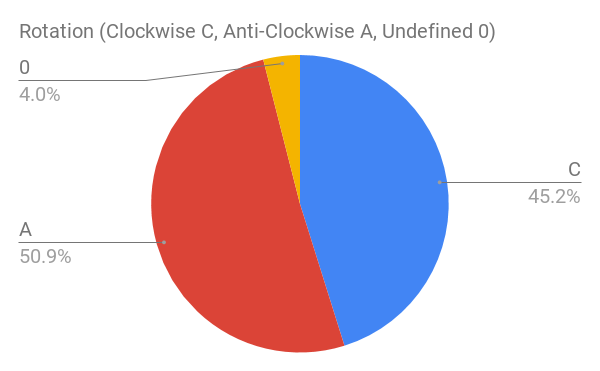
\includegraphics[scale=0.5]{images/framework/x_rotation.png}}
      \caption{Results of the manual annotation for the rotation of letter X drawings over the whole dataset. Almost half the writers drew X clockwise, the other half anti-clockwise. The undefined styles were unclear to determine.}
      \label{fig:x_rotation}
  \end{figure}

  \begin{figure}[htbp!]
      \centering
      \fbox{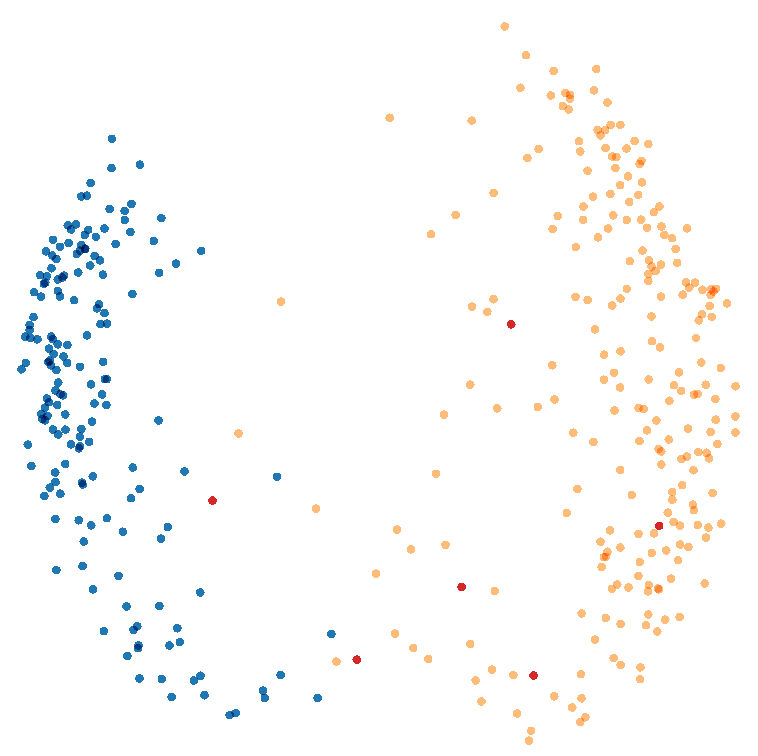
\includegraphics[scale=0.26]{images/framework/x_bottleneck.png}}
      \caption{Projection for latent space for letter X using PCA. The colors show the ground truth of the X rotation: blue is counter clockwise, orange is clockwise, and the few red points are undefined.}
      \label{fig:x_bottleneck}
  \end{figure}

  \begin{figure}[!htbp]
      \centering
      \begin{subfigure}{0.45\textwidth}
          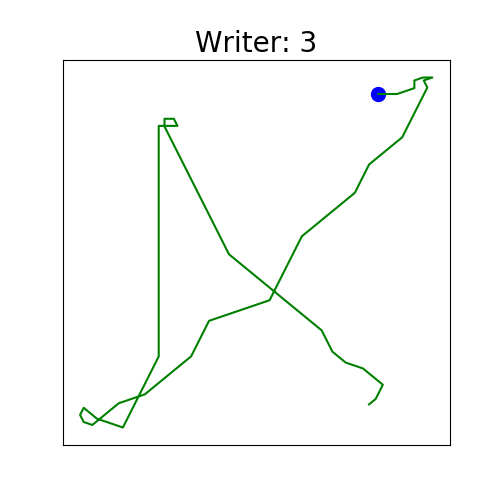
\includegraphics[scale=0.50]{images/framework/X_3.png}
      \end{subfigure}
      \hspace{0.5em}
      \begin{subfigure}{0.45\textwidth}
          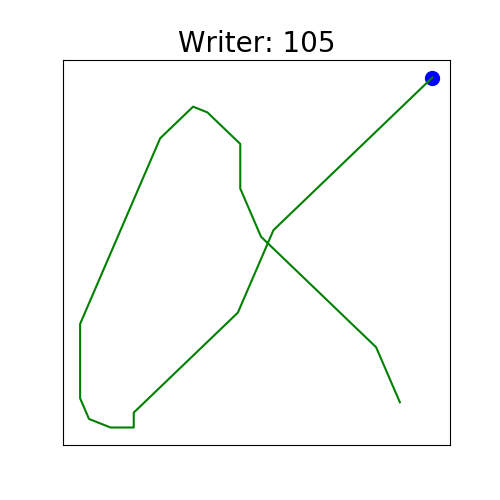
\includegraphics[scale=0.50]{images/framework/X_105.png}
      \end{subfigure}
      \vspace{1em}
      \begin{subfigure}{0.45\textwidth}
          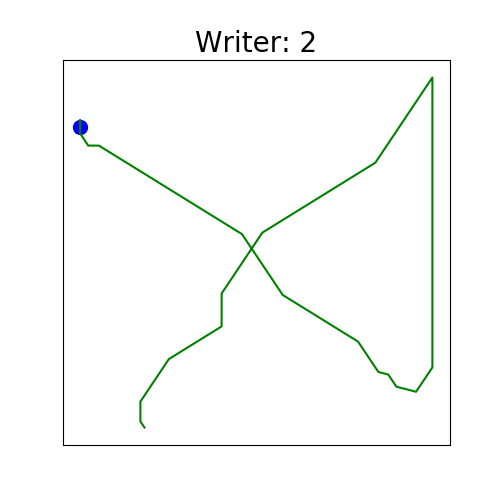
\includegraphics[scale=0.50]{images/framework/X_2.png}
      \end{subfigure}
      \hspace{0.5em}
      \begin{subfigure}{0.45\textwidth}
          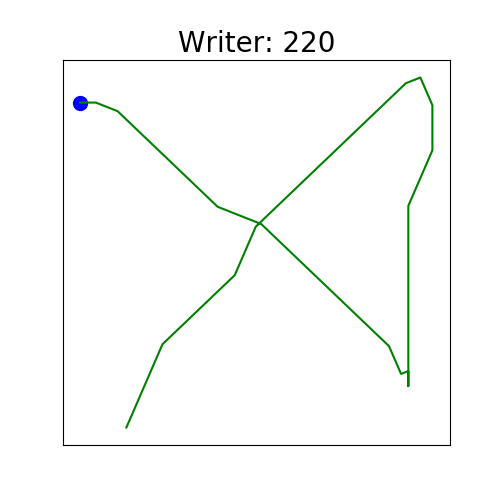
\includegraphics[scale=0.50]{images/framework/X_220.png}
      \end{subfigure}

      \caption{Examples for writing of letter X. Starting point is marked with the blue mark. Each raw is randomly sampled from each cluster in the bottleneck. The clusters shows that almost half the writers draw the letter clockwise (first row, first cluster), and the other half draw it anti-clockwise (second row, second cluster).}
      \label{fig:examples_x}
  \end{figure}

  \begin{figure}[htbp!]
      \centering
      \fbox{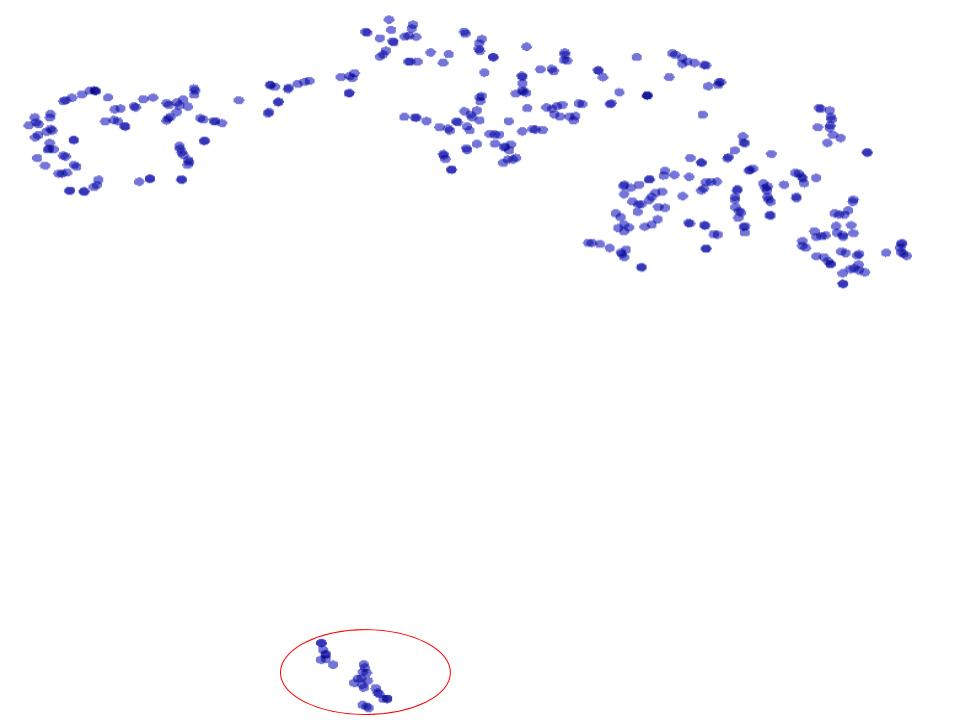
\includegraphics[scale=0.40]{images/framework/Cletter_2.jpg}}
      \caption{Projection for latent space for letter C using t-SNE. The cluster surrounded by the red circle has a clear interpretation, where writers have a cursive style.}
      \label{fig:c_letter}
  \end{figure}

  % \begin{figure}[htbp!]
  % \centering
  % \fbox{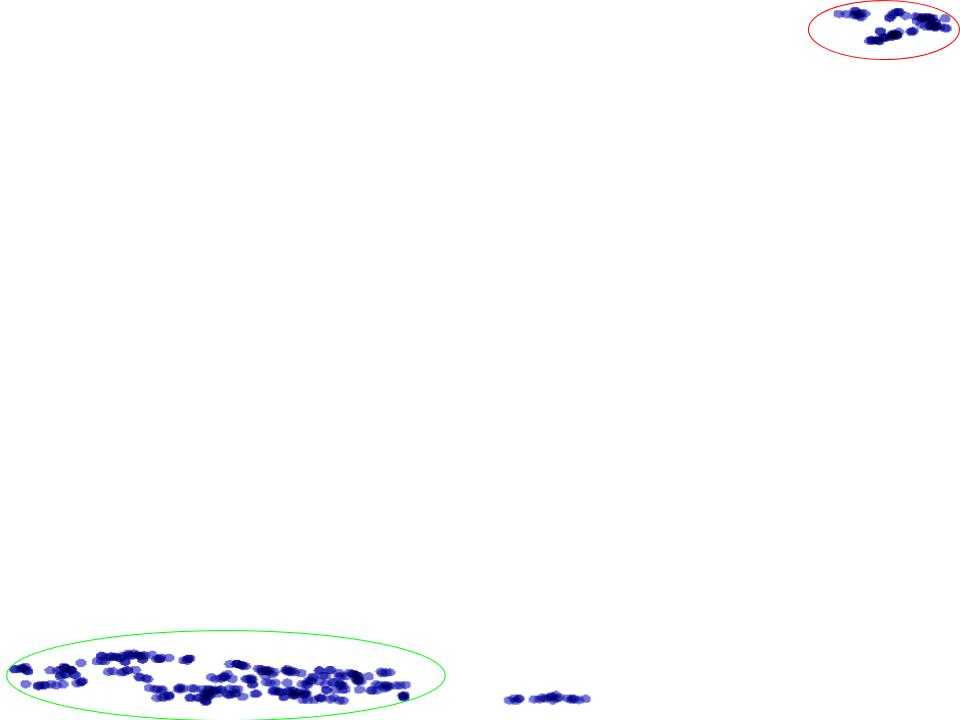
\includegraphics[scale=0.20]{a_bottleneck.jpg}}
  % \caption{Projection for bottlenecks for letter A using t-SNE.}
  % \label{fig:a_bottleneck}
  % \end{figure}

  \begin{figure}[htbp!]
      \centering
      \fbox{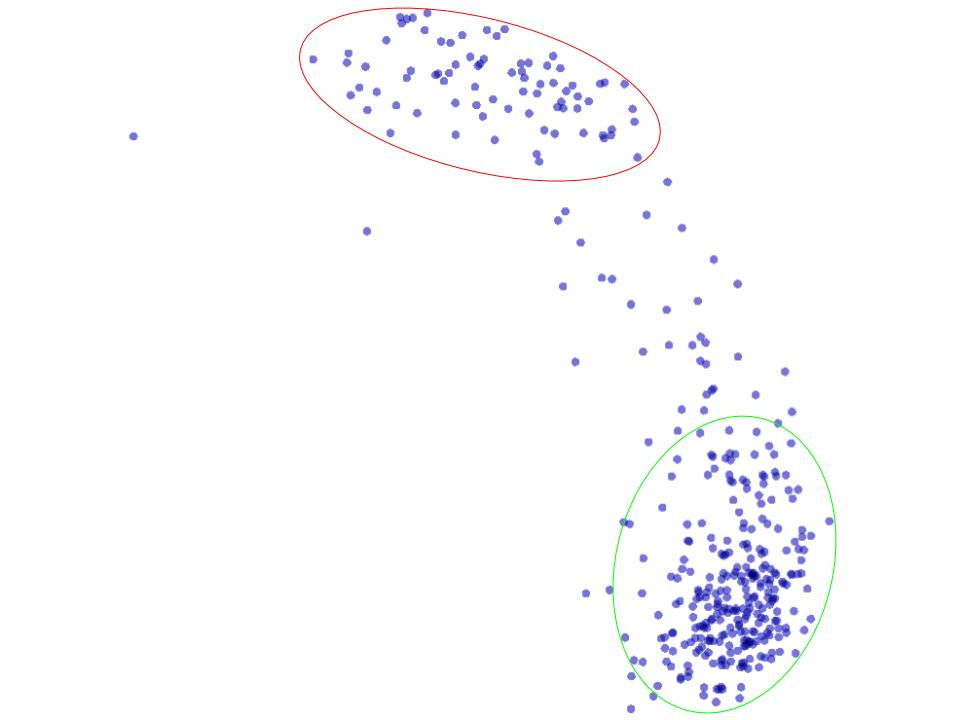
\includegraphics[scale=0.40]{images/framework/comparison_figures/letter_a_bottleneck.jpg}}
      \caption{Projection for latent space for letter A using PCA.}
      \label{fig:a_bottleneck}
  \end{figure}

  \begin{figure}[!htbp]
      \centering
      \begin{subfigure}{0.45\textwidth}
          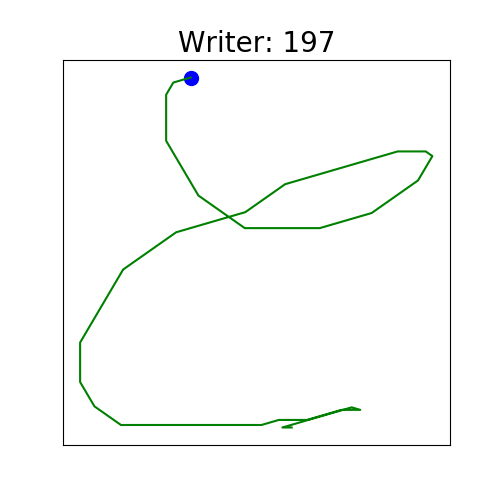
\includegraphics[scale=0.50]{images/framework/C_197.png}
      \end{subfigure}
      ~
      \begin{subfigure}{0.45\textwidth}
          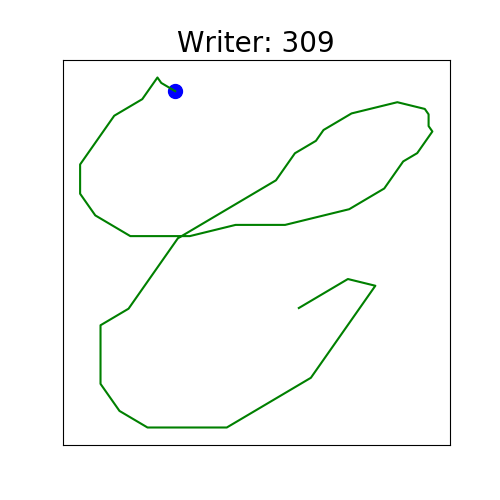
\includegraphics[scale=0.50]{images/framework/C_309.png}
      \end{subfigure}
      ~
      \begin{subfigure}{0.45\textwidth}
          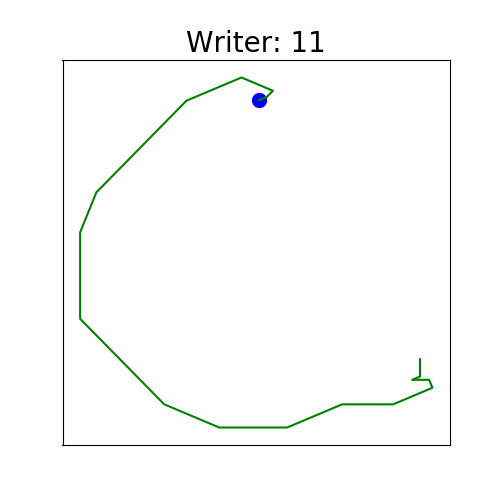
\includegraphics[scale=0.50]{images/framework/C_11.png}
      \end{subfigure}
      ~
      \begin{subfigure}{0.45\textwidth}
          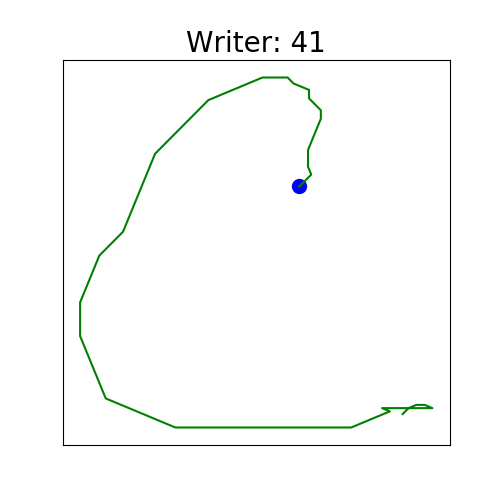
\includegraphics[scale=0.50]{images/framework/C_41.png}
      \end{subfigure}

      \caption{Examples for writing of letter C from the selected cluster (first row) versus the rest of the letter drawings (second row). Starting point is marked with the blue mark. The drawings from the selected cluster show people with Edwardian style of handwriting.}
      \label{fig:examples_c}
  \end{figure}

  \begin{figure}[!htbp]
      \centering
      \begin{subfigure}{0.45\textwidth}
          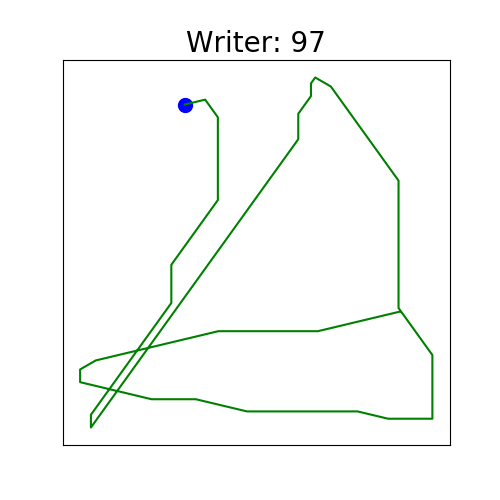
\includegraphics[scale=0.50]{images/framework/A_97.png}
      \end{subfigure}
      ~
      \begin{subfigure}{0.45\textwidth}
          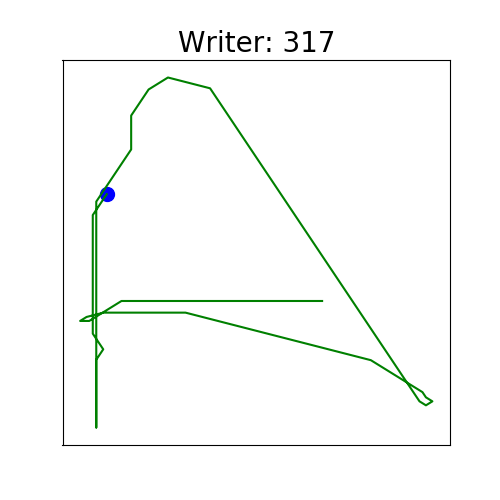
\includegraphics[scale=0.50]{images/framework/A_317.png}
      \end{subfigure}
      ~
      \begin{subfigure}{0.45\textwidth}
          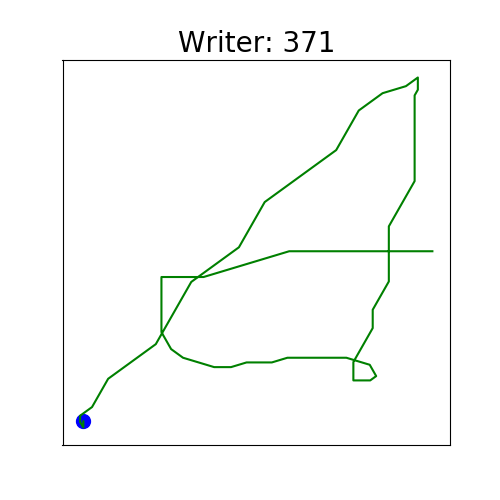
\includegraphics[scale=0.50]{images/framework/A_371.png}
      \end{subfigure}
      ~
      \begin{subfigure}{0.45\textwidth}
          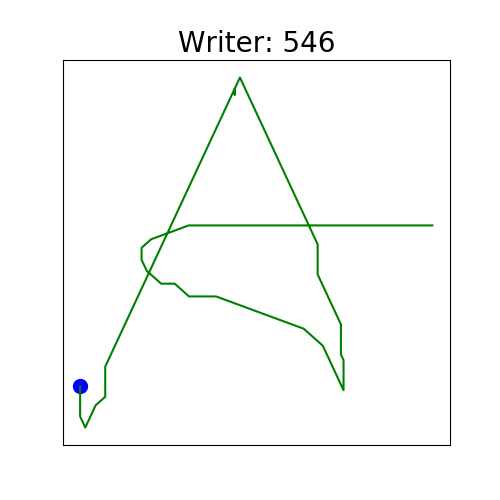
\includegraphics[scale=0.50]{images/framework/A_546.png}
      \end{subfigure}

      \caption{Examples for writing of letter A from the selected clusters. Starting point is marked with the blue mark. Each row is from one cluster. The first row show people who start drawing the letter from the top, going down, and then continue the drawing of the letter. The second row show people who start drawing from down directly.}
      \label{fig:examples_a}
  \end{figure}

  \begin{figure}[htbp!]
  \centering
  \fbox{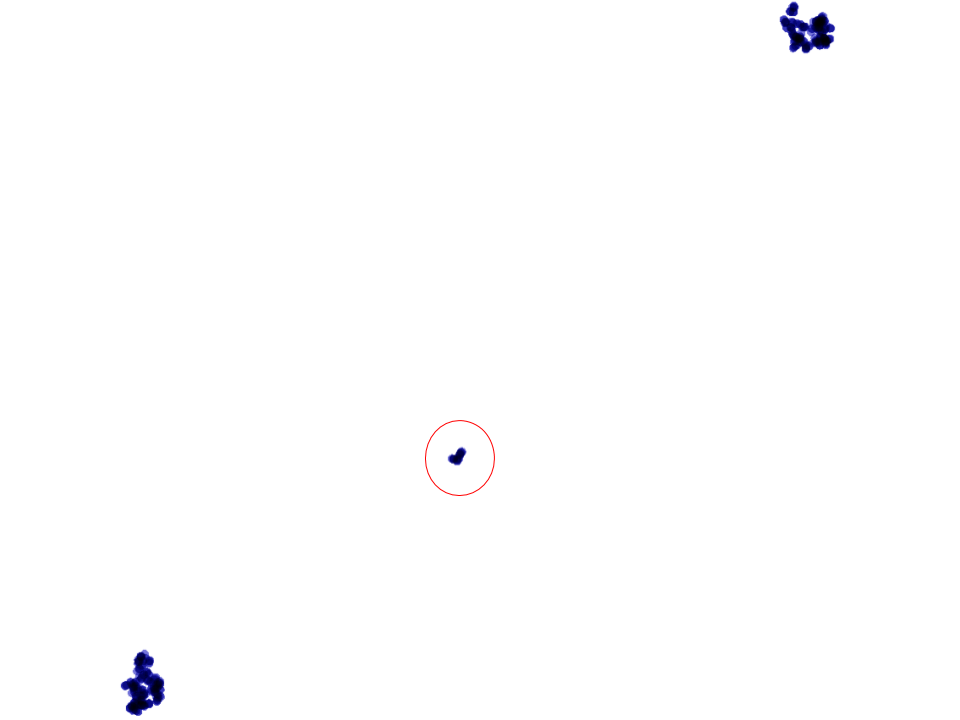
\includegraphics[scale=0.40]{images/framework/s_bottleneck.png}}
  \caption{Projection for latent space for letter S using t-SNE. We manage to interpret the indicated cluster as the Edwardian style in drawing. The other two clusters (not indicated) did not show clear difference in the style, but this is an expected behavior from using the t-SNE algorithm, since it does not try to cluster styles as an objective.}
  \label{fig:s_bottleneck}
  \end{figure}


  \begin{figure}[!htbp]
      \centering
      \begin{subfigure}{0.45\textwidth}
          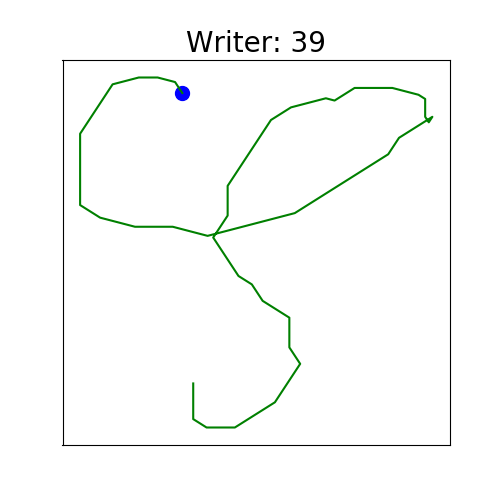
\includegraphics[scale=0.50]{images/framework/S_39.png}
      \end{subfigure}
      ~
      \begin{subfigure}{0.45\textwidth}
          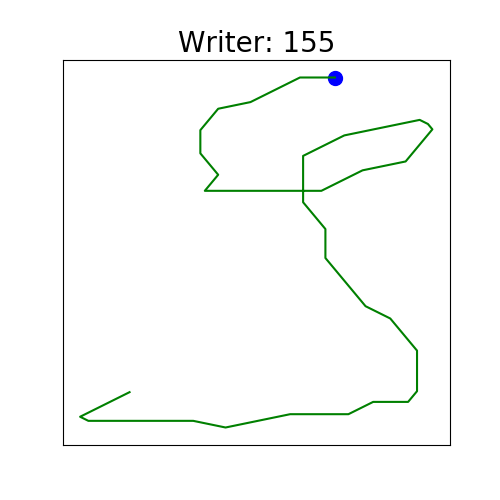
\includegraphics[scale=0.50]{images/framework/S_155.png}
      \end{subfigure}
      ~
      \begin{subfigure}{0.45\textwidth}
          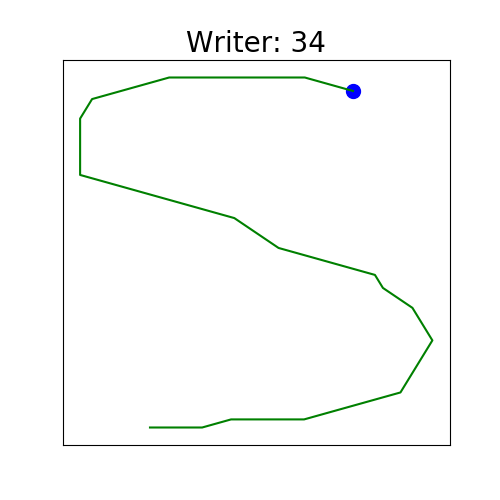
\includegraphics[scale=0.50]{images/framework/S_34.png}
      \end{subfigure}
      ~
      \begin{subfigure}{0.45\textwidth}
          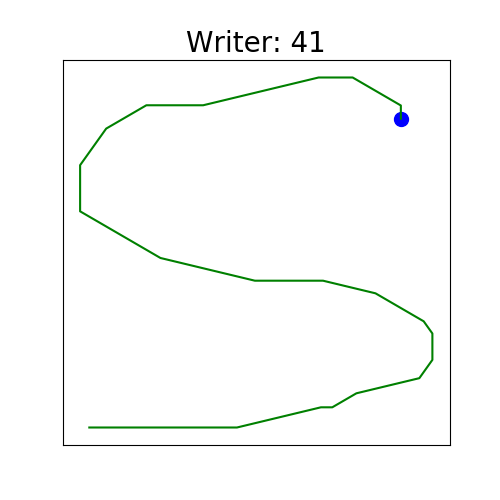
\includegraphics[scale=0.50]{images/framework/S_41.png}
      \end{subfigure}

      \caption{Examples for writing of letter S from the selected cluster (first row) versus the other two clusters (second row). Starting point is marked with the blue mark. The drawings from the selected cluster is always Edwardian style.}
      \label{fig:examples_s}
  \end{figure}

  \begin{sidewaysfigure}[!htbp]
  \centering
      \begin{subfigure}[b]{0.17\textwidth}
          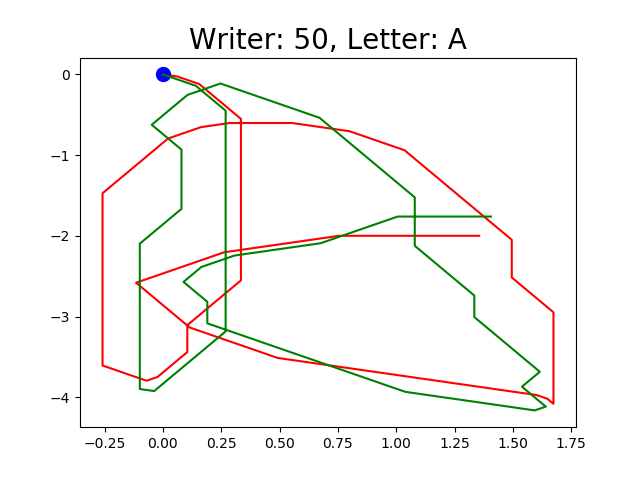
\includegraphics[width=\textwidth]{images/framework/comparison_figures/A_50.png}
      \end{subfigure}
      ~ %add desired spacing between images, e. g. ~, \quad, \qquad, \hfill etc.
        %(or a blank line to force the subfigure onto a new line)
      \begin{subfigure}[b]{0.17\textwidth}
          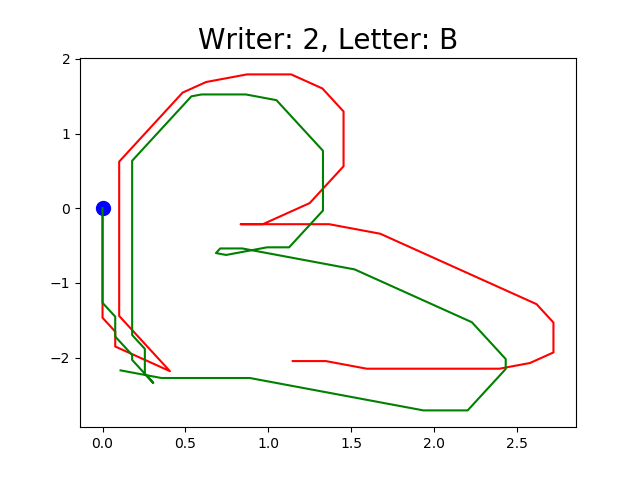
\includegraphics[width=\textwidth]{images/framework/comparison_figures/B_2.png}
      \end{subfigure}
      ~
      \begin{subfigure}[b]{0.17\textwidth}
          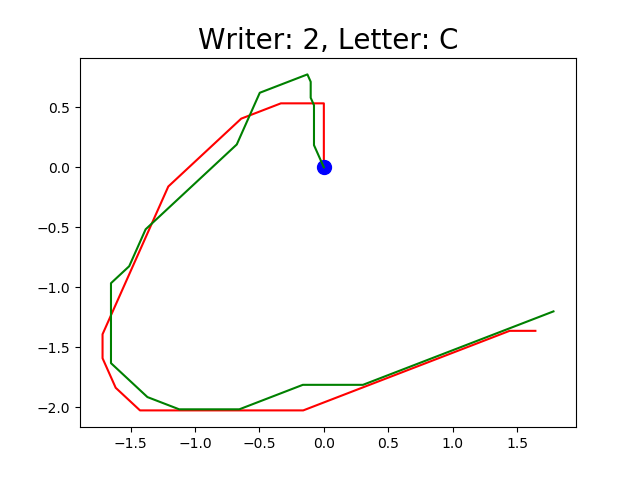
\includegraphics[width=\textwidth]{images/framework/comparison_figures/C_2.png}
      \end{subfigure}
      ~
      \begin{subfigure}[b]{0.17\textwidth}
          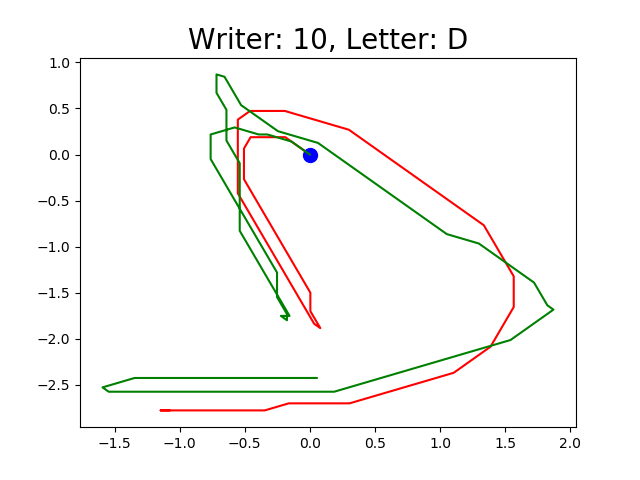
\includegraphics[width=\textwidth]{images/framework/comparison_figures/D_10.png}
      \end{subfigure}
      ~
      \begin{subfigure}[b]{0.17\textwidth}
          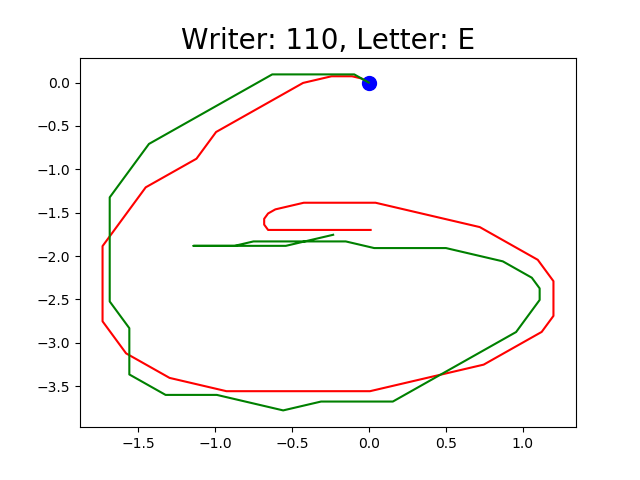
\includegraphics[width=\textwidth]{images/framework/comparison_figures/E_110.png}
      \end{subfigure}
      ~
      \begin{subfigure}[b]{0.17\textwidth}
          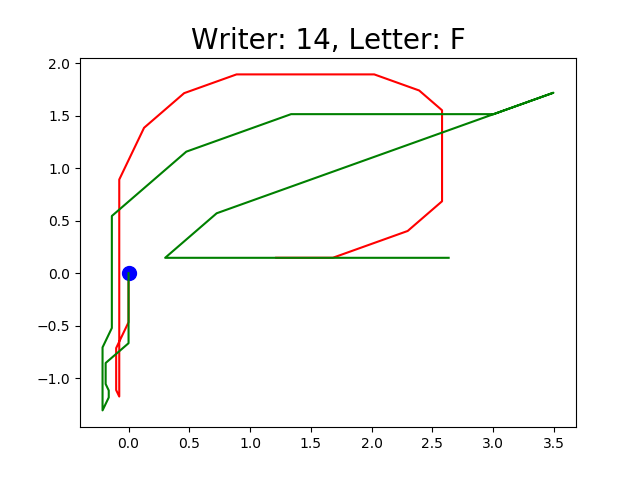
\includegraphics[width=\textwidth]{images/framework/comparison_figures/F_14.png}
      \end{subfigure}
      ~
      \begin{subfigure}[b]{0.17\textwidth}
          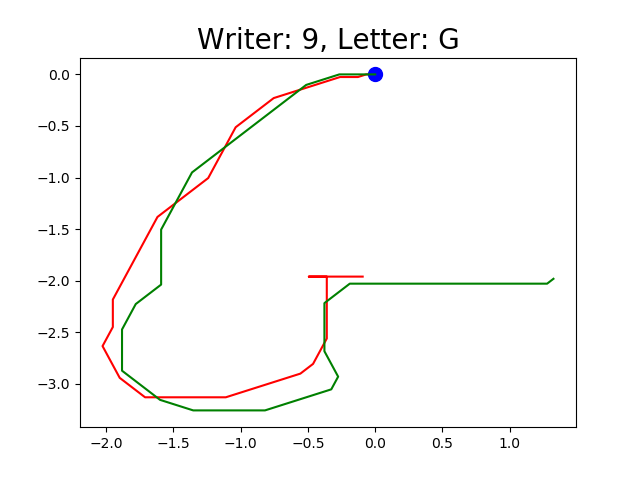
\includegraphics[width=\textwidth]{images/framework/comparison_figures/G_9.png}
      \end{subfigure}
      ~
      \begin{subfigure}[b]{0.17\textwidth}
          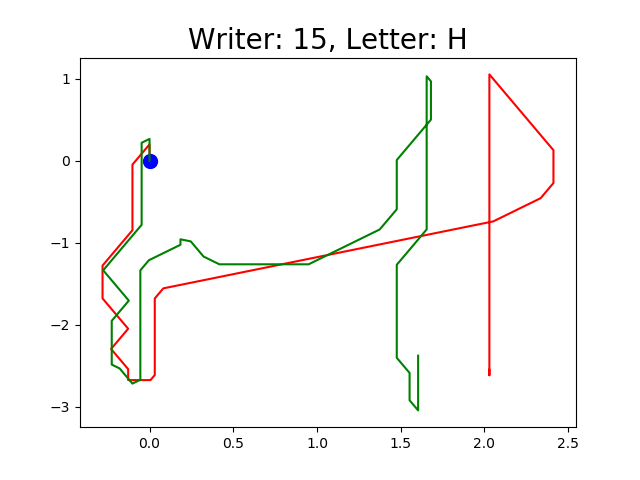
\includegraphics[width=\textwidth]{images/framework/comparison_figures/H_15.png}
      \end{subfigure}
      ~
      \begin{subfigure}[b]{0.17\textwidth}
          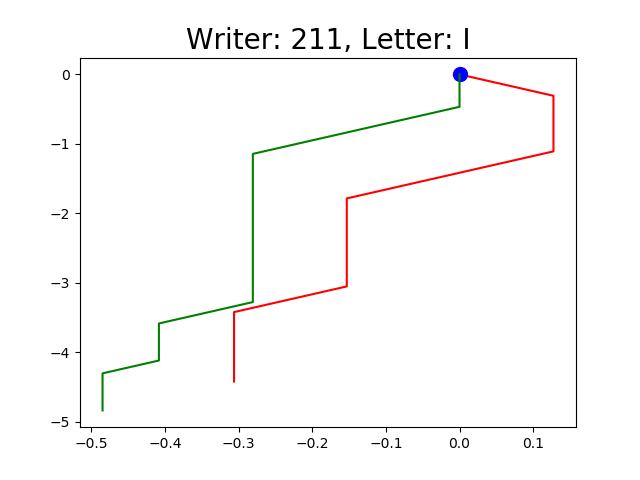
\includegraphics[width=\textwidth]{images/framework/comparison_figures/I_211.png}
      \end{subfigure}
      ~
      \begin{subfigure}[b]{0.17\textwidth}
          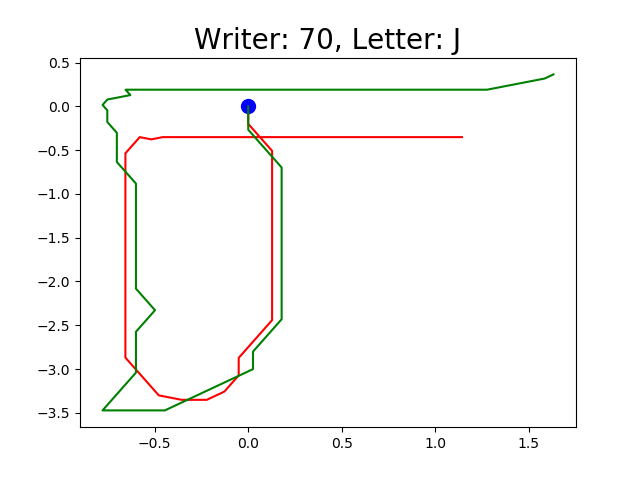
\includegraphics[width=\textwidth]{images/framework/comparison_figures/J_70.png}
      \end{subfigure}
      ~
      \begin{subfigure}[b]{0.17\textwidth}
          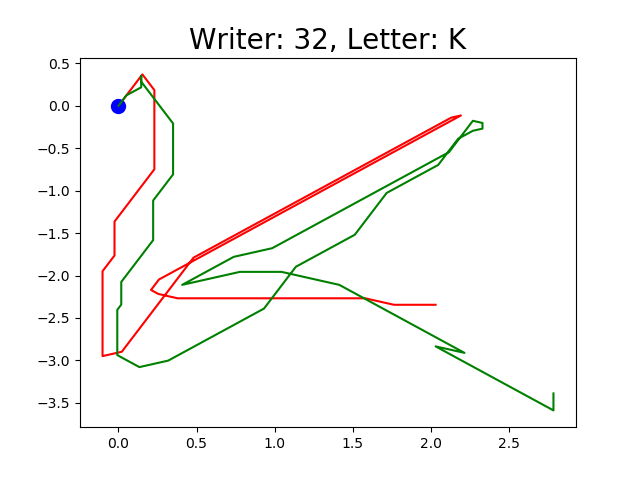
\includegraphics[width=\textwidth]{images/framework/comparison_figures/K_32.png}
      \end{subfigure}
      ~
      \begin{subfigure}[b]{0.17\textwidth}
          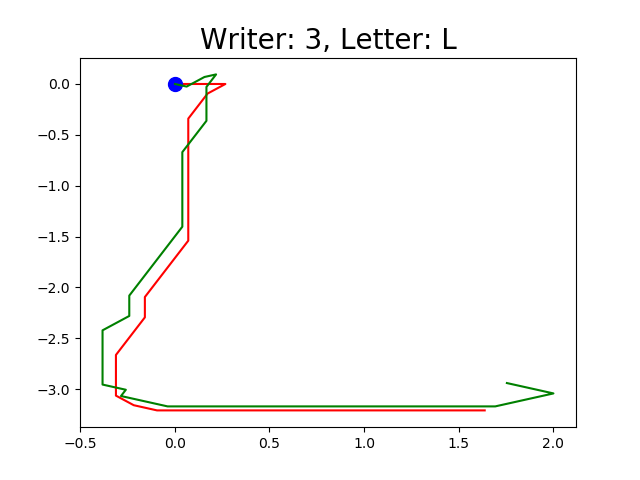
\includegraphics[width=\textwidth]{images/framework/comparison_figures/L_3.png}
      \end{subfigure}
      ~
      \begin{subfigure}[b]{0.17\textwidth}
          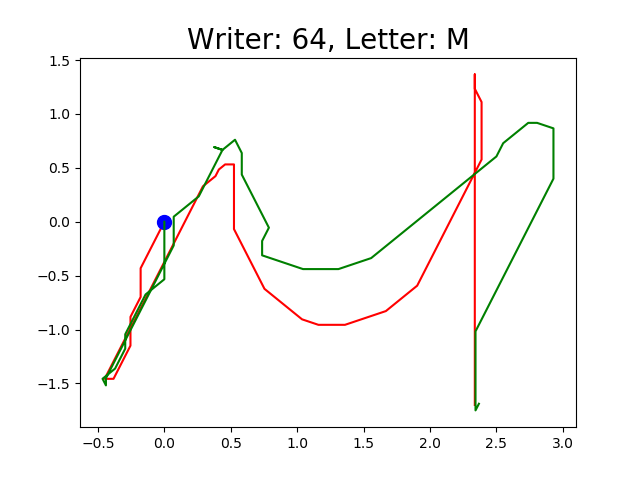
\includegraphics[width=\textwidth]{images/framework/comparison_figures/M_64.png}
      \end{subfigure}
      ~
      \begin{subfigure}[b]{0.17\textwidth}
          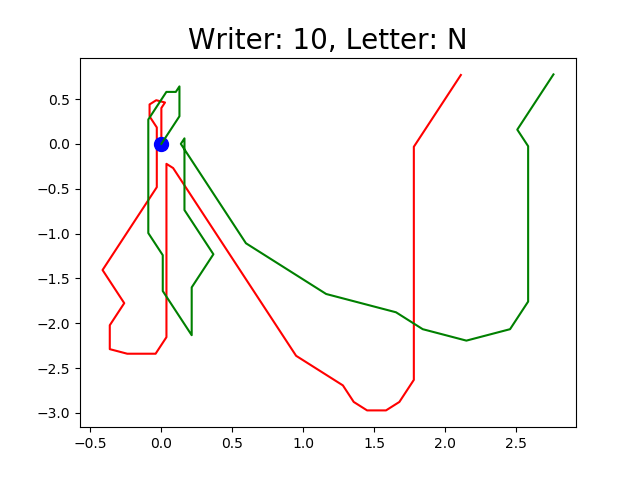
\includegraphics[width=\textwidth]{images/framework/comparison_figures/N_10.png}
      \end{subfigure}
      ~
      \begin{subfigure}[b]{0.17\textwidth}
          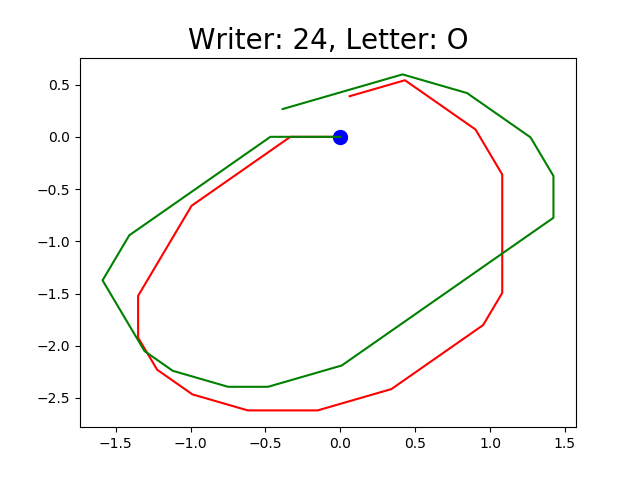
\includegraphics[width=\textwidth]{images/framework/comparison_figures/O_24.png}
      \end{subfigure}
      ~
      \begin{subfigure}[b]{0.17\textwidth}
          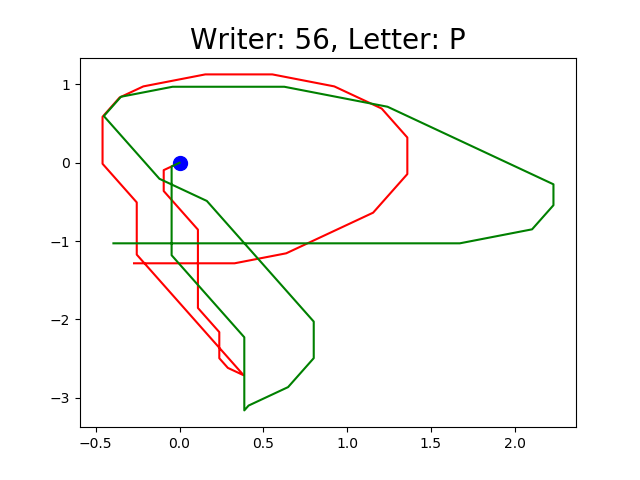
\includegraphics[width=\textwidth]{images/framework/comparison_figures/P_56.png}
      \end{subfigure}
      ~
      \begin{subfigure}[b]{0.17\textwidth}
          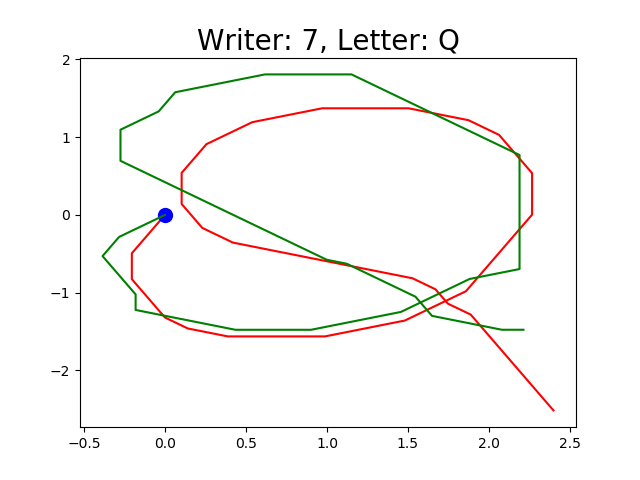
\includegraphics[width=\textwidth]{images/framework/comparison_figures/Q_7.png}
      \end{subfigure}
      ~
      \begin{subfigure}[b]{0.17\textwidth}
          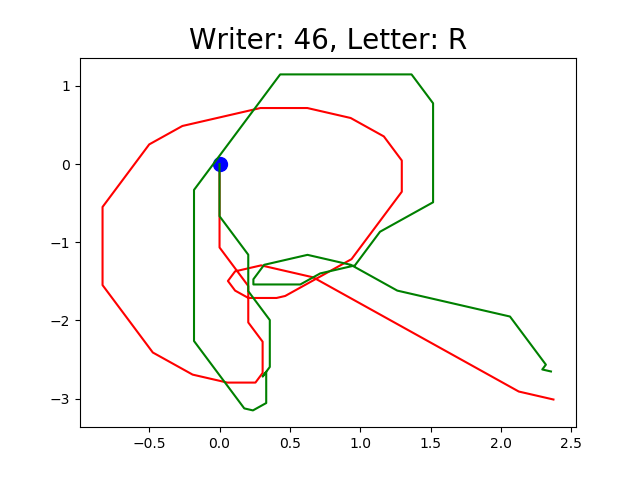
\includegraphics[width=\textwidth]{images/framework/comparison_figures/R_46.png}
      \end{subfigure}
      ~
      \begin{subfigure}[b]{0.17\textwidth}
          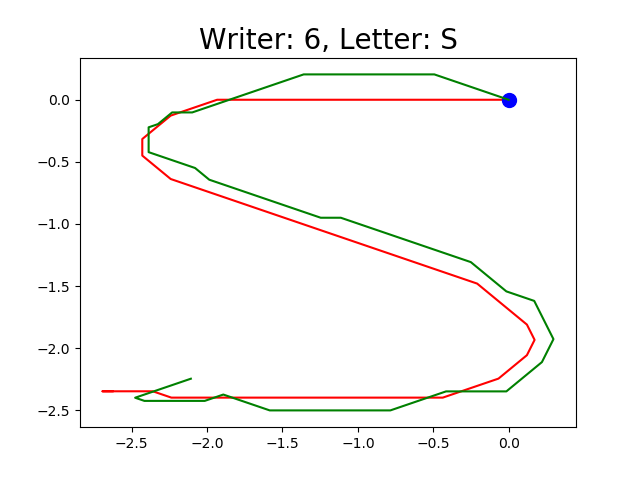
\includegraphics[width=\textwidth]{images/framework/comparison_figures/S_6.png}
      \end{subfigure}
      ~
      \begin{subfigure}[b]{0.17\textwidth}
          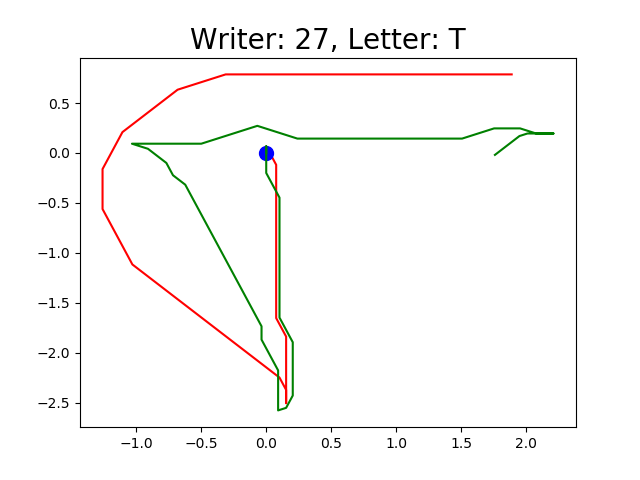
\includegraphics[width=\textwidth]{images/framework/comparison_figures/T_27.png}
      \end{subfigure}
      ~
      \begin{subfigure}[b]{0.17\textwidth}
          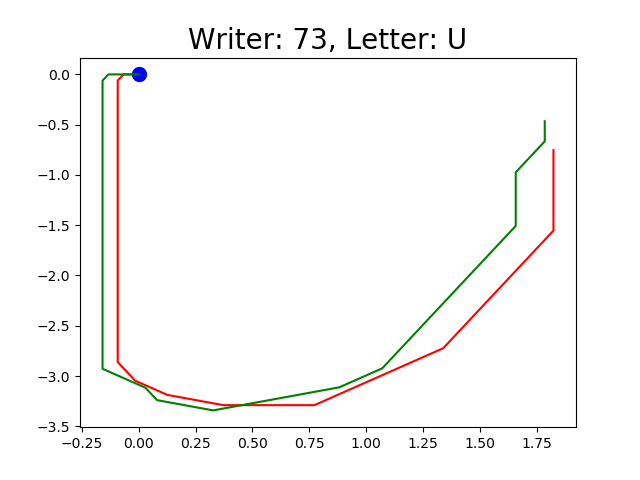
\includegraphics[width=\textwidth]{images/framework/comparison_figures/U_73.png}
      \end{subfigure}
      ~
      \begin{subfigure}[b]{0.17\textwidth}
          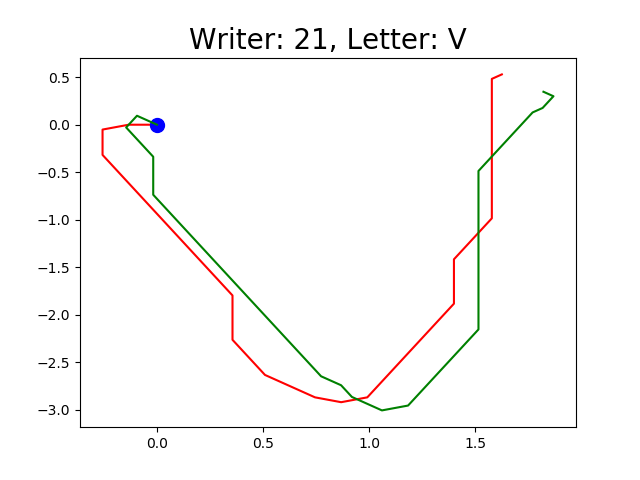
\includegraphics[width=\textwidth]{images/framework/comparison_figures/V_21.png}
      \end{subfigure}
      ~
      \begin{subfigure}[b]{0.17\textwidth}
          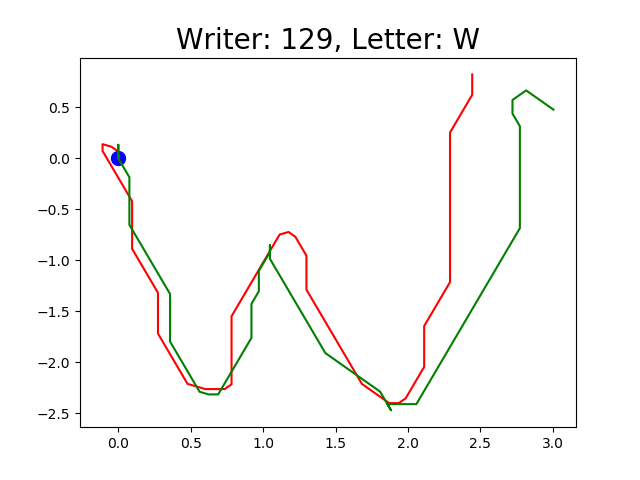
\includegraphics[width=\textwidth]{images/framework/comparison_figures/W_129.png}
      \end{subfigure}
      ~
      \begin{subfigure}[b]{0.17\textwidth}
          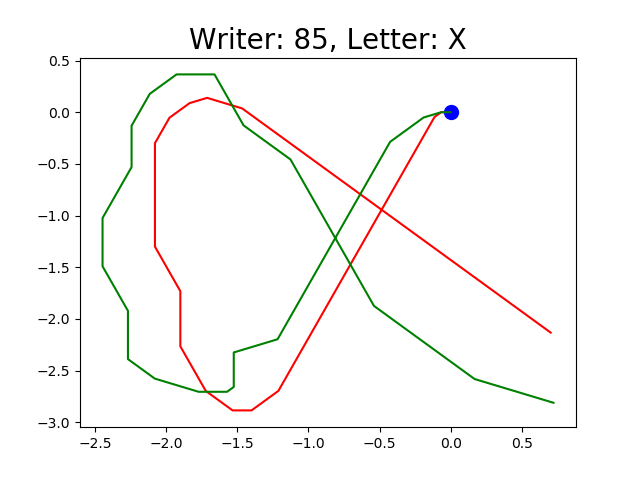
\includegraphics[width=\textwidth]{images/framework/comparison_figures/X_85.png}
      \end{subfigure}
      ~
      \begin{subfigure}[b]{0.17\textwidth}
          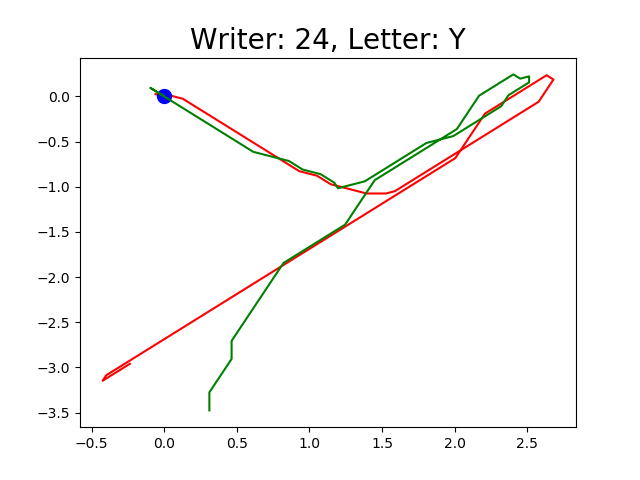
\includegraphics[width=\textwidth]{images/framework/comparison_figures/Y_24.png}
      \end{subfigure}
      ~
      \begin{subfigure}[b]{0.17\textwidth}
          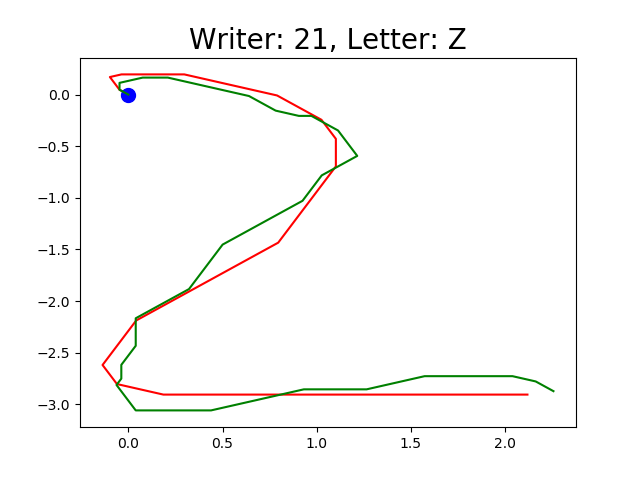
\includegraphics[width=\textwidth]{images/framework/comparison_figures/Z_21.png}
      \end{subfigure}

      %%%%%%%%%%%%%%%%%%%%%%%%5
      %%%%%%%%%%%%%%%%%%%%%%%%%%%
      \caption{Examples of generated letters. The blue mark is the starting point. The traces in green is the ground truth, and the red is the generated ones by our model.}
      \label{fig:letters_examples}
  \end{sidewaysfigure}

  \begin{sidewaysfigure}[!htbp]
  \centering
      \begin{subfigure}[b]{0.17\textwidth}
          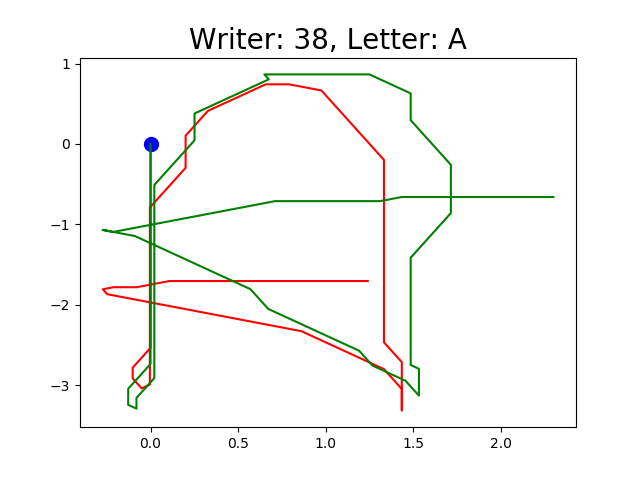
\includegraphics[width=\textwidth]{images/framework/comparison_figures/A_38.png}
      \end{subfigure}
      ~
      \begin{subfigure}[b]{0.17\textwidth}
          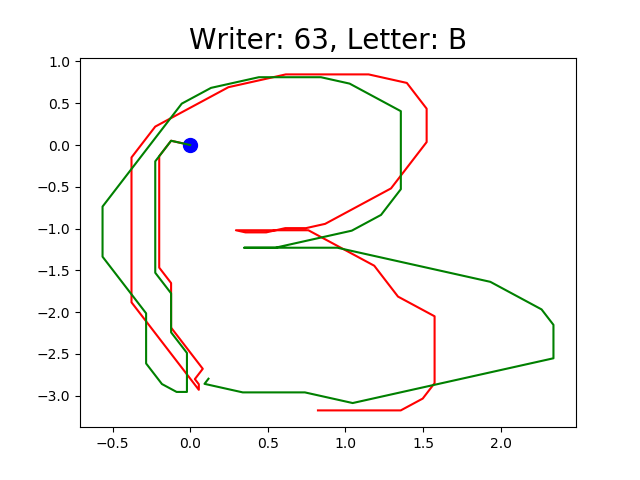
\includegraphics[width=\textwidth]{images/framework/comparison_figures/B_63.png}
      \end{subfigure}
      ~
      \begin{subfigure}[b]{0.17\textwidth}
          \includegraphics[width=\textwidth]{images/framework/comparison_figures/C_19.png}
      \end{subfigure}
      ~
      \begin{subfigure}[b]{0.17\textwidth}
          \includegraphics[width=\textwidth]{images/framework/comparison_figures/D_109.png}
      \end{subfigure}
      ~
      \begin{subfigure}[b]{0.17\textwidth}
          \includegraphics[width=\textwidth]{images/framework/comparison_figures/E_44.png}
      \end{subfigure}
      ~
      \begin{subfigure}[b]{0.17\textwidth}
          \includegraphics[width=\textwidth]{images/framework/comparison_figures/F_111.png}
      \end{subfigure}
      ~
      \begin{subfigure}[b]{0.17\textwidth}
          \includegraphics[width=\textwidth]{images/framework/comparison_figures/G_35.png}
      \end{subfigure}
      ~
      \begin{subfigure}[b]{0.17\textwidth}
          \includegraphics[width=\textwidth]{images/framework/comparison_figures/H_196.png}
      \end{subfigure}
      ~
      \begin{subfigure}[b]{0.17\textwidth}
          \includegraphics[width=\textwidth]{images/framework/comparison_figures/I_384.png}
      \end{subfigure}
      ~
      \begin{subfigure}[b]{0.17\textwidth}
          \includegraphics[width=\textwidth]{images/framework/comparison_figures/J_279.png}
      \end{subfigure}
      ~
      \begin{subfigure}[b]{0.17\textwidth}
          \includegraphics[width=\textwidth]{images/framework/comparison_figures/K_301.png}
      \end{subfigure}
      ~
      \begin{subfigure}[b]{0.17\textwidth}
          \includegraphics[width=\textwidth]{images/framework/comparison_figures/L_24.png}
      \end{subfigure}
      ~
      \begin{subfigure}[b]{0.17\textwidth}
          \includegraphics[width=\textwidth]{images/framework/comparison_figures/M_193.png}
      \end{subfigure}
      ~
      \begin{subfigure}[b]{0.17\textwidth}
          \includegraphics[width=\textwidth]{images/framework/comparison_figures/N_21.png}
      \end{subfigure}
      ~
      \begin{subfigure}[b]{0.17\textwidth}
          \includegraphics[width=\textwidth]{images/framework/comparison_figures/O_38.png}
      \end{subfigure}
      ~
      \begin{subfigure}[b]{0.17\textwidth}
          \includegraphics[width=\textwidth]{images/framework/comparison_figures/P_65.png}
      \end{subfigure}
      ~
      \begin{subfigure}[b]{0.17\textwidth}
          \includegraphics[width=\textwidth]{images/framework/comparison_figures/Q_140.png}
      \end{subfigure}
      ~
      \begin{subfigure}[b]{0.17\textwidth}
          \includegraphics[width=\textwidth]{images/framework/comparison_figures/R_91.png}
      \end{subfigure}
      ~
      \begin{subfigure}[b]{0.17\textwidth}
          \includegraphics[width=\textwidth]{images/framework/comparison_figures/S_125.png}
      \end{subfigure}
      ~
      \begin{subfigure}[b]{0.17\textwidth}
          \includegraphics[width=\textwidth]{images/framework/comparison_figures/T_84.png}
      \end{subfigure}
      ~
      \begin{subfigure}[b]{0.17\textwidth}
          \includegraphics[width=\textwidth]{images/framework/comparison_figures/U_83.png}
      \end{subfigure}
      ~
      \begin{subfigure}[b]{0.17\textwidth}
          \includegraphics[width=\textwidth]{images/framework/comparison_figures/V_32.png}
      \end{subfigure}
      ~
      \begin{subfigure}[b]{0.17\textwidth}
          \includegraphics[width=\textwidth]{images/framework/comparison_figures/W_191.png}
      \end{subfigure}
      ~
      \begin{subfigure}[b]{0.17\textwidth}
          \includegraphics[width=\textwidth]{images/framework/comparison_figures/X_187.png}
      \end{subfigure}
      ~
      \begin{subfigure}[b]{0.17\textwidth}
          \includegraphics[width=\textwidth]{images/framework/comparison_figures/Y_61.png}
      \end{subfigure}
      ~
      \begin{subfigure}[b]{0.17\textwidth}
          \includegraphics[width=\textwidth]{images/framework/comparison_figures/Z_383.png}
      \end{subfigure}
      %%%%%%%%%%%%%%%%%%%%%%%%5
      %%%%%%%%%%%%%%%%%%%%%%%%%%%
      \caption{Examples of generated letters. The blue mark is the starting point. The traces in green is the ground truth, and the red is the generated ones by our model.}
      \label{fig:letters_examples_2}
  \end{sidewaysfigure}
